% =====================================================================================================
% From the Metadata Guidelines to curation actions: auditing the semantic artefacts of EarthPortal
% Emmanuel Nyandu Kagarabi, internship at CNRS / Data Terra (1 September to 31 October 2026)
%
% OntoPortal Federation meeting, 13 November 2026, 9:30 to 10:30 (about 35 minutes of talk, then discussion)
%
% Compile with pdfLaTeX (TeX Live, Overleaf):  latexmk -pdf emmanuel_dataTerra_Slides_2026-11-13_EditorialBoard.tex
% or with XeLaTeX:                            latexmk -xelatex emmanuel_dataTerra_Slides_2026-11-13_EditorialBoard.tex
% (the PDF delivered on 11 November 2026 was compiled with XeLaTeX and the Lato font)
% Clean auxiliary files: latexmk -C emmanuel_dataTerra_Slides_2026-11-13_EditorialBoard.tex
%
% Figures:  ../earthportal_sa_audit/figures/ (fig_*.pdf, saved by notebooks 03 and 05, snapshot of
%           10 November 2026), Figures/slides_2026-11-13/ (screenshots of the audits, snapshots of
%           10 November 2026, logos, Earth picture, QR codes) and Figures/ (CNRS and SISSA logos).
%           Compile from docs/ so that every path is found.
% =====================================================================================================
\documentclass[aspectratio=169,10pt]{beamer}

% ---- Font: Lato (falls back to Helvetica with pdfLaTeX if the lato package is missing) ---------------
\usepackage{iftex}
\ifPDFTeX
  \usepackage[T1]{fontenc}
  \usepackage[utf8]{inputenc}
  \IfFileExists{lato.sty}{\usepackage[default]{lato}}{\usepackage[scaled=0.95]{helvet}}
\else
  \usepackage{fontspec}
  \setmainfont{Lato}
  \setsansfont{Lato}
\fi
\usefonttheme[onlymath]{serif}

\usepackage{amsmath}
\usepackage{booktabs}
\usepackage{tabularx}
\usepackage{tikz}
\usetikzlibrary{arrows.meta,positioning,fit,calc}
\usepackage{qrcode}
\usepackage{hyperref}

% ---- Colours (the same as the TIB slides) -------------------------------------------------------------
\definecolor{epnavy}{HTML}{2A2058}
\definecolor{epink}{HTML}{1B2A2F}
\definecolor{epgrey}{HTML}{6B7B80}
\definecolor{epteal}{HTML}{3E8E7E}
\definecolor{epblue}{HTML}{1F4E9C}
\definecolor{epmid}{HTML}{2E6FC4}
\definecolor{eplight}{HTML}{4A8FE0}
\definecolor{epcard}{HTML}{EEF4F2}
\definecolor{epsky}{HTML}{EAF1FB}
\definecolor{epred}{HTML}{A4303F}
% Names used in the frames of the first version of this deck, mapped to the new colours
\colorlet{dtnavy}{epnavy}
\colorlet{dtteal}{epteal}
\colorlet{dtindigo}{epmid}
\colorlet{dtred}{epred}
\colorlet{dtband}{epcard}
\colorlet{dtgrey}{epgrey}
\colorlet{dtink}{epink}

% ---- The theme: title at the top, footer with the logos, cards for the blocks ---------------------------
\setbeamertemplate{navigation symbols}{}
\setbeamercolor{normal text}{fg=epink}
\setbeamercolor{frametitle}{fg=epnavy}
\setbeamerfont{frametitle}{size=\fontsize{17}{20}\selectfont,series=\bfseries}
\setbeamercolor{alerted text}{fg=epred}
\setbeamercolor{structure}{fg=epblue}
\setbeamertemplate{itemize item}{\color{epblue}\raisebox{0.15ex}{\scriptsize$\bullet$}}
\setbeamertemplate{itemize subitem}{\color{epgrey}\raisebox{0.15ex}{\tiny$\bullet$}}
\setbeamertemplate{enumerate items}[circle]
\setbeamercolor{item projected}{fg=white,bg=epnavy}

% Blocks are drawn as the cards of the TIB slides: a light card with a bold coloured heading
\setbeamercolor{block body}{bg=epcard,fg=epink}
\setbeamercolor{block body alerted}{bg=epcard,fg=epink}
\setbeamercolor{block body example}{bg=epcard,fg=epink}
\setbeamercolor{block title}{fg=epnavy}
\setbeamercolor{block title alerted}{fg=epred}
\setbeamercolor{block title example}{fg=epteal}
\setbeamerfont{block title}{series=\bfseries,size=\normalsize}
\setbeamertemplate{blocks}[rounded][shadow=false]
\setbeamertemplate{block begin}{\par\vskip\medskipamount
  \begin{beamercolorbox}[rounded=true,shadow=false,leftskip=7pt,rightskip=7pt,vmode]{block body}
  \vskip5pt{\usebeamerfont{block title}\usebeamercolor[fg]{block title}\insertblocktitle\par}\vskip3pt}
\setbeamertemplate{block end}{\vskip5pt\end{beamercolorbox}\vskip\smallskipamount}
\setbeamertemplate{block alerted begin}{\par\vskip\medskipamount
  \begin{beamercolorbox}[rounded=true,shadow=false,leftskip=7pt,rightskip=7pt,vmode]{block body alerted}
  \vskip5pt{\usebeamerfont{block title}\usebeamercolor[fg]{block title alerted}\insertblocktitle\par}\vskip3pt}
\setbeamertemplate{block alerted end}{\vskip5pt\end{beamercolorbox}\vskip\smallskipamount}
\setbeamertemplate{block example begin}{\par\vskip\medskipamount
  \begin{beamercolorbox}[rounded=true,shadow=false,leftskip=7pt,rightskip=7pt,vmode]{block body example}
  \vskip5pt{\usebeamerfont{block title}\usebeamercolor[fg]{block title example}\insertblocktitle\par}\vskip3pt}
\setbeamertemplate{block example end}{\vskip5pt\end{beamercolorbox}\vskip\smallskipamount}

% The row of our logos, in one order everywhere: the host institution (CNRS), the research
% infrastructure (Data Terra), the portal it runs (EarthPortal), then my university (SISSA).
\newcommand{\logorow}[1]{% #1 = scale (1 on the title page)
  
\includegraphics[height=#1\dimexpr 0.62cm\relax]{Figures/Logo_CNRS-fr.png}\hspace{#1\dimexpr 0.55cm\relax}%
  
\includegraphics[height=#1\dimexpr 0.62cm\relax]{Figures/slides_2026-11-13/Logo_DATATERRA_mark.png}\hspace{#1\dimexpr 0.55cm\relax}%
  
\includegraphics[height=#1\dimexpr 0.50cm\relax]{Figures/slides_2026-11-13/EarthPortal_logo_pill.png}\hspace{#1\dimexpr 0.55cm\relax}%
  
\includegraphics[height=#1\dimexpr 0.85cm\relax]{Figures/Logo_SISSA-it.png}}
\newcommand{\meetingline}{OntoPortal Federation Meeting, 13 November 2026}

\newif\ifshownumber\shownumbertrue
% Footer of the content slides: logos on the left, meeting and page number on the right
\setbeamertemplate{background}{%
  \begin{tikzpicture}[remember picture,overlay]
    \draw[epcard,line width=0.8pt] ($(current page.south west)+(0.5cm,0.98cm)$) -- ($(current page.south east)+(-0.5cm,0.98cm)$);
    \node[anchor=south west,inner sep=0pt] at ($(current page.south west)+(0.55cm,0.13cm)$) {\logorow{0.85}};
    \node[anchor=south east,text=epgrey,font=\scriptsize,inner sep=0pt] at ($(current page.south east)+(-1.25cm,0.36cm)$) {\meetingline};
    \ifshownumber\node[anchor=south east,text=epgrey,font=\scriptsize,inner sep=0pt] at ($(current page.south east)+(-0.55cm,0.36cm)$) {\insertframenumber};\fi
  \end{tikzpicture}}
\setbeamertemplate{frametitle}{\vspace*{0.45cm}\hspace*{0.35cm}\insertframetitle}
\setbeamersize{text margin left=0.9cm,text margin right=0.9cm}
% Keep the bottom 1 cm free for the footer drawn in the background
\setbeamertemplate{footline}{\vskip1.0cm}

% Dark frames (title and thank you): the Earth picture, cut at the bottom to leave a white band
\newcommand{\darkbackground}{%
  \setbeamertemplate{background}{%
    \begin{tikzpicture}[remember picture,overlay]
      \node[anchor=north,inner sep=0pt] at (current page.north)
        {
\includegraphics[width=\paperwidth]{Figures/slides_2026-11-13/earth_background.jpg}};
      \fill[white] (current page.south west) rectangle ($(current page.south east)+(0,1.7cm)$);
      \node[inner sep=0pt] at ($(current page.south)+(0,0.85cm)$) {\logorow{1.3}};
      \node[anchor=north west,inner sep=0pt] at (current page.north west)
        {
\includegraphics[width=3.6cm]{Figures/slides_2026-11-13/EarthPortal_logo.png}};
    \end{tikzpicture}}}

\tikzset{
  num/.style={circle,fill=#1,text=white,font=\Large\bfseries,minimum size=1.05cm,inner sep=0pt},
  card/.style={rounded corners=8pt,fill=epcard,draw=none},
  pill/.style={rounded corners=5pt,fill=#1,text=white,font=\small\bfseries,align=center,inner sep=5pt},
  arr/.style={-{Stealth[length=2.6mm]},epgrey,line width=0.9pt}}

% Section pages: the number of the part in a circle, its title, and where we are among the six parts
\newcommand{\partcolour}[1]{\ifcase#1\or epnavy\or epblue\or epmid\or eplight\or epteal\or epgrey\fi}
\AtBeginSection[]{%
  {\shownumberfalse
  \begin{frame}[noframenumbering]
    \centering
    \begin{tikzpicture}
      \node[num=\partcolour{\thesection},minimum size=1.6cm,font=\fontsize{26}{28}\selectfont\bfseries] (n) at (0,0) {\thesection};
      \node[text=epnavy,font=\fontsize{22}{26}\selectfont\bfseries,anchor=north] at (0,-1.15) {\insertsectionhead};
      \foreach \i in {1,...,6} {
        \ifnum\i=\thesection
          \node[circle,fill=\partcolour{\i},minimum size=0.32cm,inner sep=0pt] at (\i*0.55-1.925,-2.75) {};
        \else
          \node[circle,draw=epgrey!60,line width=0.6pt,minimum size=0.26cm,inner sep=0pt] at (\i*0.55-1.925,-2.75) {};
        \fi}
    \end{tikzpicture}
  \end{frame}}}

\newcommand{\evidence}[1]{{\scriptsize\color{epgrey}#1}}
\newcommand{\code}[1]{\texttt{\small #1}}
\newcommand{\bignum}[2]{{\color{#2}\fontsize{26}{28}\selectfont\bfseries #1}}

% No hyphenation: short texts read better on slides
\hyphenpenalty=10000
\exhyphenpenalty=10000

\begin{document}

% =====================================================================================================
% Title
{\darkbackground
\begin{frame}[plain,noframenumbering]
  \begin{tikzpicture}[remember picture,overlay]
    \node[text=white,font=\fontsize{24}{28}\selectfont\bfseries,align=center] at ($(current page.center)+(0,1.55cm)$)
      {From the Metadata Guidelines\\to curation actions};
    \node[text=white,font=\large,align=center] at ($(current page.center)+(0,0.3cm)$)
      {Auditing the semantic artefacts of EarthPortal with your guidelines and O'FAIRe};
    \node[text=white,font=\normalsize\itshape,align=center] at ($(current page.center)+(0,-0.55cm)$)
      {Emmanuel Nyandu Kagarabi};
    \node[text=white!85,font=\footnotesize,align=center] at ($(current page.center)+(0,-1.05cm)$)
      {Internship at CNRS / Data Terra, 1 September to 31 October 2026 \quad Supervisor: Christelle Pierkot};
    \node[text=white,font=\small\bfseries,align=center] at ($(current page.south)+(0,2.15cm)$)
      {\meetingline};
  \end{tikzpicture}
\end{frame}
}

% -----------------------------------------------------------------------------------------------------
\begin{frame}{Today: 35 minutes of talk, then discussion}
  \begin{columns}[c]
    \begin{column}{0.47\textwidth}
      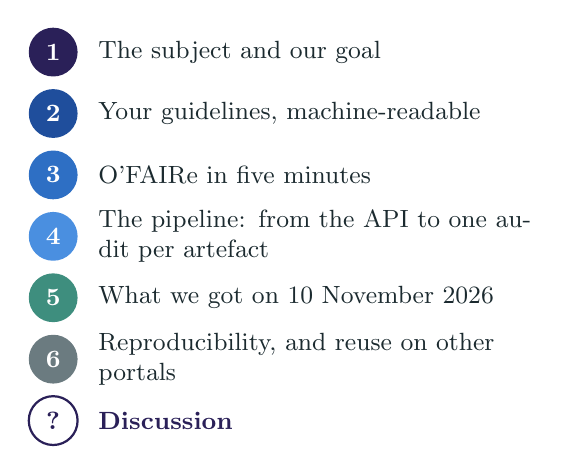
\begin{tikzpicture}
        \foreach \i/\c/\t in {1/epnavy/{The subject and our goal}, 2/epblue/{Your guidelines, machine-readable},
                              3/epmid/{O'FAIRe in five minutes}, 4/eplight/{The pipeline: from the API to one audit per artefact},
                              5/epteal/{What we got on 10 November 2026}, 6/epgrey/{Reproducibility, and reuse on other portals}} {
          \node[num=\c,minimum size=0.62cm,font=\small\bfseries] at (0,-\i*0.78) {\i};
          \node[anchor=west,text=epink,font=\small,text width=5.6cm] at (0.45,-\i*0.78) {\t};
        }
        \node[circle,draw=epnavy,line width=0.8pt,minimum size=0.62cm,font=\small\bfseries,text=epnavy] at (0,-7*0.78) {?};
        \node[anchor=west,text=epnavy,font=\small\bfseries] at (0.45,-7*0.78) {Discussion};
      \end{tikzpicture}
    \end{column}
    \begin{column}{0.49\textwidth}
      \begin{exampleblock}{The message of this talk}
        Your Metadata Guidelines became a \textbf{table that a program can read}. With it, and with
        O'FAIRe as a measuring instrument, every artefact of EarthPortal now has an
        \textbf{audit}: what is missing, what it costs, and who can fix it.
      \end{exampleblock}
      \vspace{4pt}
      \evidence{Everything shown today is open and citable: SA\_Management v1.0.0,
      \href{https://doi.org/10.5281/zenodo.23417011}{doi.org/10.5281/zenodo.23417011}.}
    \end{column}
  \end{columns}
\end{frame}

% =====================================================================================================
\section{The subject and our goal}

% -----------------------------------------------------------------------------------------------------
\begin{frame}{Where we started}
  \centering
  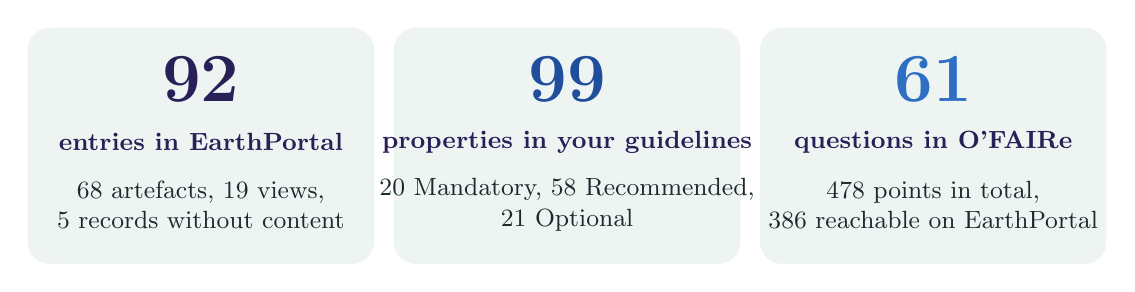
\begin{tikzpicture}
    \foreach \x/\c/\n/\head/\body in {
      -4.65/epnavy/92/{entries in EarthPortal}/{68 artefacts, 19 views,\\5 records without content},
       0.00/epblue/99/{properties in your guidelines}/{20 Mandatory, 58 Recommended,\\21 Optional},
       4.65/epmid/61/{questions in O'FAIRe}/{478 points in total,\\386 reachable on EarthPortal}} {
      \node[card,minimum width=4.4cm,minimum height=3.0cm] at (\x,0.6) {};
      \node[text=\c,font=\fontsize{28}{30}\selectfont\bfseries] at (\x,1.45) {\n};
      \node[text=epnavy,font=\small\bfseries] at (\x,0.65) {\head};
      \node[text=epink,font=\small,align=center] at (\x,-0.15) {\body};
    }
  \end{tikzpicture}\\[2pt]
  \begin{block}{Two references, one catalogue}
    \small The guidelines say \textbf{what a good description contains}; O'FAIRe \textbf{scores} how FAIR
    an artefact is from its description. EarthPortal stores the descriptions in \textbf{130 fields}
    (110 per submission, 20 per ontology record). Our work connects the three.
  \end{block}
  \evidence{Snapshot of 10 November 2026. Guidelines: review version of September 2026, the base of our cheatsheet (Report 1).}
\end{frame}

% -----------------------------------------------------------------------------------------------------
\begin{frame}{Our goal}
  \begin{columns}[c]
    \begin{column}{0.55\textwidth}
      For each artefact of EarthPortal, answer three questions:
      \begin{enumerate}
        \item \textbf{What is missing} in its description, according to the guidelines?
        \item \textbf{What does it cost} in FAIRness, according to O'FAIRe?
        \item \textbf{Who can fix it}: the author, the curator, or the portal?
      \end{enumerate}
      \vspace{6pt}
      And do it \textbf{again and again}: each run is a dated snapshot, so we can follow the catalogue
      over time.
    \end{column}
    \begin{column}{0.42\textwidth}
      \begin{alertblock}{What we do not do}
        \small We do not change O'FAIRe. We use it \textbf{as an instrument}. But to read its scores
        correctly, we read its Java code
        (\href{https://github.com/agroportal/fairness/}{\code{agroportal/fairness}}, commit \code{24def6b}).
      \end{alertblock}
      \vspace{4pt}
      \begin{block}{Who it is for}
        \small Authors (their audit), curators (the actions), and you: what the catalogue says about
        the guidelines.
      \end{block}
    \end{column}
  \end{columns}
\end{frame}

% =====================================================================================================
\section{Your guidelines, machine-readable}

% -----------------------------------------------------------------------------------------------------
\begin{frame}{From a document to a machine-readable table}
  \centering
  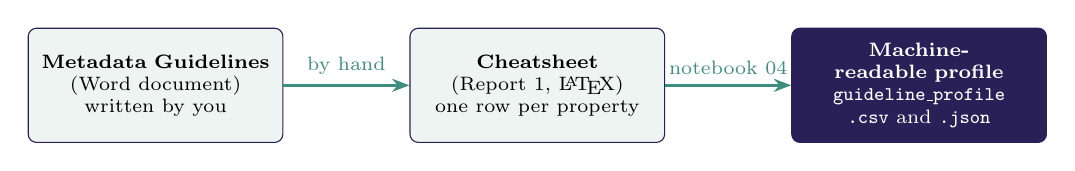
\begin{tikzpicture}[font=\scriptsize,
      doc/.style={draw=dtnavy, rounded corners=3pt, fill=dtband, minimum height=1.45cm, text width=3.0cm, align=center},
      arr/.style={-{Stealth[length=2.2mm]}, dtteal, line width=1pt}]
    \node[doc] (g) {\textbf{Metadata Guidelines}\\(Word document)\\written by you};
    \node[doc, right=1.6cm of g] (c) {\textbf{Cheatsheet}\\(Report 1, \LaTeX)\\one row per property};
    \node[doc, right=1.6cm of c, fill=dtnavy, text=white] (p) {\textbf{Machine-readable profile}\\\texttt{guideline\_profile}\\\texttt{.csv} and \texttt{.json}};
    \draw[arr] (g) -- node[above]{by hand} (c);
    \draw[arr] (c) -- node[above]{notebook 04} (p);
  \end{tikzpicture}\\[4pt]
  \begin{columns}[T]
    \begin{column}{0.50\textwidth}
      \small
      \textbf{One row of the profile} (property 1.9):\\[3pt]
      \scriptsize
      \begin{tabular}{@{}l l@{}}
        \toprule
        id, section & 1.9, General\\
        entry, usage & Version IRI, Recommended\\
        property (guidelines) & \code{omv:versionIRI}\\
        stored by EarthPortal as & \code{owl:versionIRI} (submission)\\
        link rule & manual\\
        who fixes it & author\\
        \bottomrule
      \end{tabular}
      \evidence{Check out \href{https://github.com/EarthPortal/SA_Management/blob/main/earthportal_sa_audit/mapping/guideline_profile.csv}{\code{guideline\_profile.csv}}.}
    \end{column}
    \begin{column}{0.46\textwidth}
      \small
      \textbf{What a program now knows}, for all 99 properties:
      \begin{itemize}
        \item its usage and FAIR principle
        \item where the portal stores it (record or submission, API key)
        \item its allowed values, when the portal has a list
        \item who can fill it: author 86, curator 8, portal 5
      \end{itemize}
      \evidence{The split author / curator / portal is our proposal, to be validated.}
    \end{column}
  \end{columns}
\end{frame}

% -----------------------------------------------------------------------------------------------------
\begin{frame}{Guidelines and portal schema: 99 / 99 linked}
  \begin{columns}[T]
    \begin{column}{0.40\textwidth}
      \small
      \begin{tabular}{@{}l l r@{}}
        \toprule
        Rule & Meaning & Properties\\
        \midrule
        \textbf{same} & same name & 72\\
        \textbf{mapping} & a declared synonym & 21\\
        \textbf{manual} & linked by hand & 6\\
        \bottomrule
      \end{tabular}
    \end{column}
    \begin{column}{0.56\textwidth}
      \small A synonym is declared in the portal schema (\texttt{metadataMappings}): for example
      \texttt{dcat:keyword} is stored as \texttt{omv:keywords}. The 21 mapped properties need nothing.
    \end{column}
  \end{columns}
  \vspace{8pt}
  {\small\textbf{Five names of the guidelines that the portal does not recognise}}\\[3pt]
  \scriptsize
  \begin{tabularx}{\textwidth}{@{}l l l X@{}}
    \toprule
    Id & Guidelines & EarthPortal field & Note\\
    \midrule
    1.1 & \texttt{mod:acronym} & \texttt{omv:acronym} (ontology record) & no synonym declared\\
    1.9 & \texttt{omv:versionIRI} & \texttt{owl:versionIRI} & MOD 3.2 uses \texttt{owl:versionIRI}: the guidelines may be the one to correct\\
    10.1 & \texttt{dct:isPartOf} & \texttt{viewOf} (ontology record) & the portal only has the inverse, \texttt{dct:hasPart}\\
    10.5 & \texttt{mod:semanticArtefactRelation} & \texttt{door:ontologyRelatedTo} & equivalent in MOD 3.2, but not listed by the portal\\
    10.10 & \texttt{mod:hasDisparateModelling} & \texttt{door:hasDisparateModelling} & the portal lists \texttt{mod:hasDisparateModellingWith}\\
    \bottomrule
  \end{tabularx}\\[4pt]
  \small If an author writes these names in the file, we expect the portal not to read them.
  \vfill
  \evidence{\href{https://github.com/EarthPortal/SA_Management/blob/main/docs/build/emmanuel_dataTerra_Report5-Cheatsheet-vs-EarthPortal.pdf}{Report 5} (October 2026). 
  Portal schema: \href{https://data.earthportal.eu/submission_metadata}{\texttt{/submission\_metadata}}, \href{https://data.earthportal.eu/ontology_metadata}{\texttt{/ontology\_metadata}}; MOD:\href{https://github.com/FAIR-IMPACT/MOD}{FAIR-IMPACT/MOD/}\texttt{mod.ttl}.}
\end{frame}

% -----------------------------------------------------------------------------------------------------
\begin{frame}{Your question of 13 October}
  \begin{columns}[T]
    \begin{column}{0.53\textwidth}
      \scriptsize
      \begin{tabular}{@{}l l@{}}
        \toprule
        EarthPortal field (label) & Read by O'FAIRe\\
        \midrule
        \texttt{omv:version} (version information) & R1.2Q4\\
        \texttt{owl:deprecated} (deprecated) & A2Q4\\
        \texttt{prefLabelProperty} (preferred label) & I3Q3, R1Q1\\
        \texttt{synonymProperty} (synonym) & I3Q3, R1Q1\\
        \texttt{definitionProperty} (definition) & I3Q3, R1Q1\\
        \texttt{authorProperty} (author) & I3Q3, R1Q1\\
        \texttt{obsoleteProperty} (obsolete) & I3Q3, R1Q1\\
        \texttt{hierarchyProperty} (hierarchy) & I3Q3, R1Q2\\
        \texttt{createdProperty} (creation date) & no\\
        \texttt{modifiedProperty} (modification date) & no\\
        \bottomrule
      \end{tabular}\\[4pt]
      {\tiny The last eight are the ``object description properties'' of the portal.}
    \end{column}
    \begin{column}{0.44\textwidth}
      \small
      \textbf{Fields read by O'FAIRe, absent from the guidelines.} \textbf{10 fields} of the schema
      are filled from the file, but no property of the guidelines points to them; \textbf{8} of them
      bring O'FAIRe points.\\[6pt]
      \begin{alertblock}{Most values are defaults}
        \scriptsize In about 55 artefacts they hold the same values. The OntoPortal code gives
        defaults: \texttt{skos:prefLabel} (even for OWL), \texttt{owl:subClassOf} for OWL hierarchies,
        \texttt{dc:created}. As far as we know, the last two do not exist in their vocabularies.
      \end{alertblock}
    \end{column}
  \end{columns}
  \vfill
  \evidence{\href{https://github.com/EarthPortal/SA_Management/blob/main/docs/build/emmanuel_dataTerra_Report5-Cheatsheet-vs-EarthPortal.pdf}{Report 5} (October 2026)}
\end{frame}

% =====================================================================================================
\section{O'FAIRe in five minutes}

% -----------------------------------------------------------------------------------------------------
\begin{frame}{What is O'FAIRe?}
  \begin{columns}[T]
    \begin{column}{0.52\textwidth}
      \small
      \textbf{O'FAIRe} (\emph{Ontology FAIRness Evaluator}) scores how FAIR a semantic artefact is,
      using \textbf{its metadata} on an OntoPortal instance.
      \begin{itemize}\setlength{\itemsep}{0pt}
        \item 4 principles $\rightarrow$ 15 sub-principles $\rightarrow$ \textbf{61 questions}
        \item each question pays credits, from 0 to its maximum $m_q$
        \item no human judgement: the same description always gets the same score
      \end{itemize}
      \footnotesize
      \begin{tabular}{@{}l c c@{}}
        \toprule
        Principle & Questions & Maximum\\
        \midrule
        Findable & 13 & 113\\
        Accessible & 13 & 113\\
        Interoperable & 15 & 109\\
        Reusable & 20 & 143\\
        \midrule
        \textbf{Total} & \textbf{61} & \textbf{478}\\
        \bottomrule
      \end{tabular}
    \end{column}
    \begin{column}{0.45\textwidth}
      \begin{block}{The score of an artefact $o$}
        \[ S(o) = \sum_{q=1}^{61} s_q(o), \qquad 0 \le s_q(o) \le m_q \]
        \[ N(o) = \left\lfloor 100 \cdot \frac{S(o)}{478} \right\rfloor \]
      \end{block}
      {\small\textbf{Example, OSO:} $S = 364.36$, so $N = \lfloor 76.2 \rfloor = 76$.}\\[2pt]
      \evidence{Amdouni, Bouazzouni \& Jonquet (2022), \emph{O\textquotesingle FAIRe makes you an offer}, IJMSO 16(1).}
    \end{column}
  \end{columns}
\end{frame}

% -----------------------------------------------------------------------------------------------------
\begin{frame}{What the 478 points measure on EarthPortal}
  \centering
  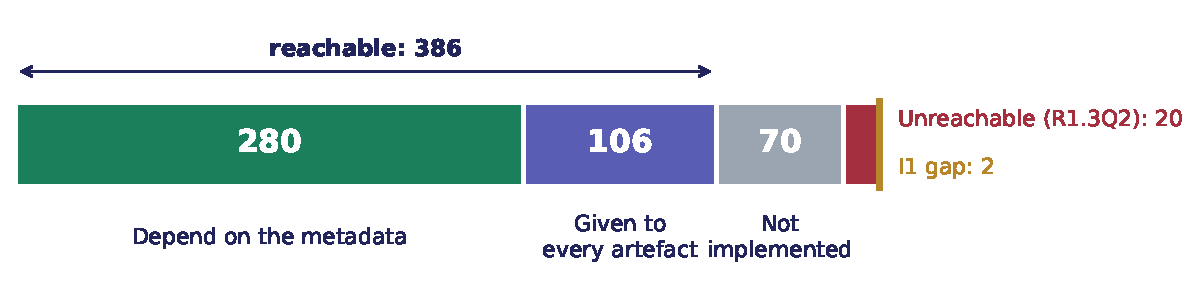
\includegraphics[width=0.97\textwidth]{../earthportal_sa_audit/figures/fig_478_split.pdf}\\[4pt]
  \begin{columns}[T]
    \begin{column}{0.52\textwidth}
      \small
      No EarthPortal artefact can earn 92 of the 478 points: 10 questions are not implemented (70),
      R1.3Q2 rewards AgroPortal and OBO groups (20), I1 counts 44 for 42 (2). So, beside O'FAIRe's
      score, we report a \textbf{reachable score}:
      \[ R(o) = 100 \cdot \frac{S(o)}{386} \]
    \end{column}
    \begin{column}{0.44\textwidth}
      \small
      \begin{tabular}{@{}l r r@{}}
        \toprule
        OSO & O'FAIRe $N$ & Reachable $R$\\
        \midrule
        & 76 / 100 & \textbf{94.4 \%}\\
        \bottomrule
      \end{tabular}\\[6pt]
      \evidence{Read from the Java code (commit \code{24def6b}). The ranking of the artefacts is the same
      with both scores; only the scale changes.}
    \end{column}
  \end{columns}
\end{frame}

% =====================================================================================================
\section{The pipeline}

% -----------------------------------------------------------------------------------------------------
\begin{frame}{Five notebooks: collect once, then compute}
  \centering
  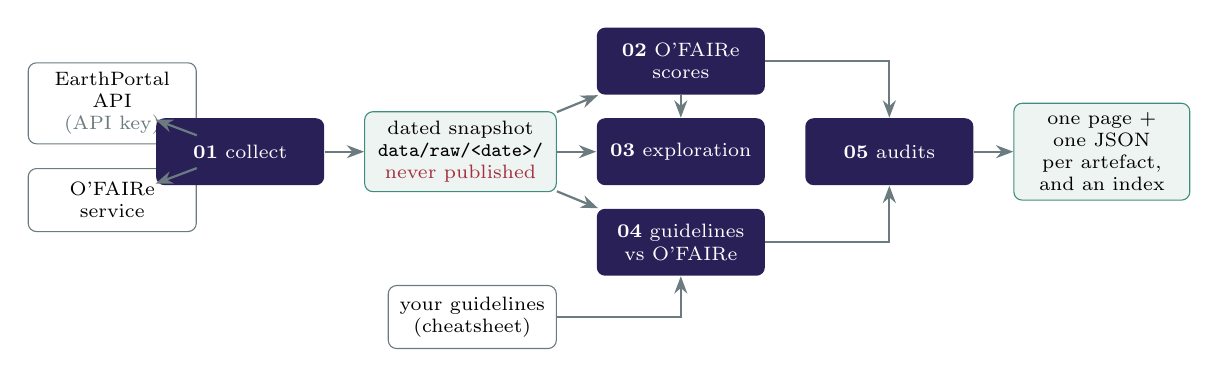
\begin{tikzpicture}[
      font=\scriptsize,
      src/.style={draw=dtgrey, rounded corners=3pt, fill=white, minimum height=0.8cm, text width=1.9cm, align=center},
      nbk/.style={draw=none, rounded corners=3pt, fill=dtnavy, text=white, minimum height=0.85cm, text width=1.9cm, align=center},
      res/.style={draw=dtteal, rounded corners=3pt, fill=dtband, minimum height=0.8cm, text width=2.2cm, align=center},
      arr/.style={-{Stealth[length=2.2mm]}, dtgrey, line width=0.8pt}]
    \node[src] (api) {EarthPortal API\\\textcolor{dtgrey}{(API key)}};
    \node[src, below=0.3cm of api] (of) {O'FAIRe service};
    \node[nbk, right=0.55cm of $(api)!0.5!(of)$] (n1) {\textbf{01} collect};
    \node[res, right=0.5cm of n1] (raw) {dated snapshot\\\texttt{data/raw/<date>/}\\\textcolor{dtred}{never published}};
    \node[nbk, right=0.5cm of raw, yshift=1.15cm] (n2) {\textbf{02} O'FAIRe scores};
    \node[nbk, right=0.5cm of raw] (n3) {\textbf{03} exploration};
    \node[nbk, right=0.5cm of raw, yshift=-1.15cm] (n4) {\textbf{04} guidelines vs O'FAIRe};
    \node[src, left=0.5cm of n4, yshift=-0.95cm] (cs) {your guidelines\\(cheatsheet)};
    \node[nbk, right=0.5cm of n3] (n5) {\textbf{05} audits};
    \node[res, right=0.5cm of n5, text width=2.0cm] (aud) {one page + one JSON per artefact, and an index};
    \draw[arr] (api) -- (n1); \draw[arr] (of) -- (n1); \draw[arr] (n1) -- (raw);
    \draw[arr] (raw) -- (n2); \draw[arr] (raw) -- (n3); \draw[arr] (raw) -- (n4);
    \draw[arr] (n2) -- (n3); \draw[arr] (cs) -| (n4);
    \draw[arr] (n2) -| (n5); \draw[arr] (n4) -| (n5); \draw[arr] (n5) -- (aud);
  \end{tikzpicture}\\[6pt]
  \scriptsize
  \begin{tabularx}{\textwidth}{@{}l X@{}}
    \textbf{01} & downloads the catalogue, the portal schema, the latest submission and the O'FAIRe result of every entry\\
    \textbf{02--03} & turn O'FAIRe's answers into one table, and explore it\\
    \textbf{04} & reads your guidelines, finds where the portal stores each property, and links each question to the properties it reads\\
    \textbf{05} & writes the audits\\
  \end{tabularx}
\end{frame}

% -----------------------------------------------------------------------------------------------------
\begin{frame}{How a lost point becomes an action}
  \centering
  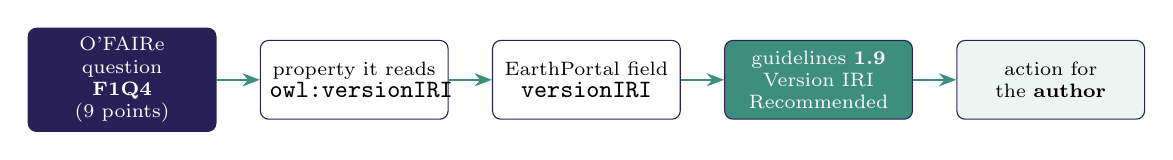
\begin{tikzpicture}[font=\scriptsize,
      box/.style={draw=dtnavy, rounded corners=3pt, fill=white, minimum height=1.0cm, text width=2.15cm, align=center},
      arr/.style={-{Stealth[length=2.2mm]}, dtteal, line width=0.9pt}]
    \node[box, fill=dtnavy, text=white] (q) {O'FAIRe question\\\textbf{F1Q4}\\(9 points)};
    \node[box, right=0.55cm of q] (p) {property it reads\\\code{owl:versionIRI}};
    \node[box, right=0.55cm of p] (f) {EarthPortal field\\\code{versionIRI}};
    \node[box, right=0.55cm of f, fill=dtteal, text=white] (c) {guidelines \textbf{1.9}\\Version IRI\\Recommended};
    \node[box, right=0.55cm of c, fill=dtband] (a) {action for\\the \textbf{author}};
    \draw[arr] (q) -- (p); \draw[arr] (p) -- (f); \draw[arr] (f) -- (c); \draw[arr] (c) -- (a);
  \end{tikzpicture}\\[10pt]
  \begin{columns}[T]
    \begin{column}{0.50\textwidth}
      \small
      Every \textbf{empty} property of the guidelines is an action. When a question loses $L_q$
      points and reads $n_q$ empty properties, each of them gets a share:
      \[ \text{share}(a) = \sum_{q \text{ reads } a} \frac{L_q}{n_q} \]
      {\scriptsize A way to rank actions, not a promise of points.}
    \end{column}
    \begin{column}{0.46\textwidth}
      \begin{block}{Priorities: guidelines first, then points}
        \small
        \begin{tabular}{@{}c l@{}}
          \textbf{P1} & Mandatory\\
          \textbf{P2} & Recommended, costs O'FAIRe points\\
          \textbf{P3} & Optional, costs O'FAIRe points\\
          P4 & Recommended\\
          P5 & Optional\\
        \end{tabular}
      \end{block}
    \end{column}
  \end{columns}
\end{frame}

% -----------------------------------------------------------------------------------------------------
\begin{frame}{One audit per artefact: 1. FAIRness}
  \begin{columns}[c]
    \begin{column}{0.68\textwidth}
      \centering
      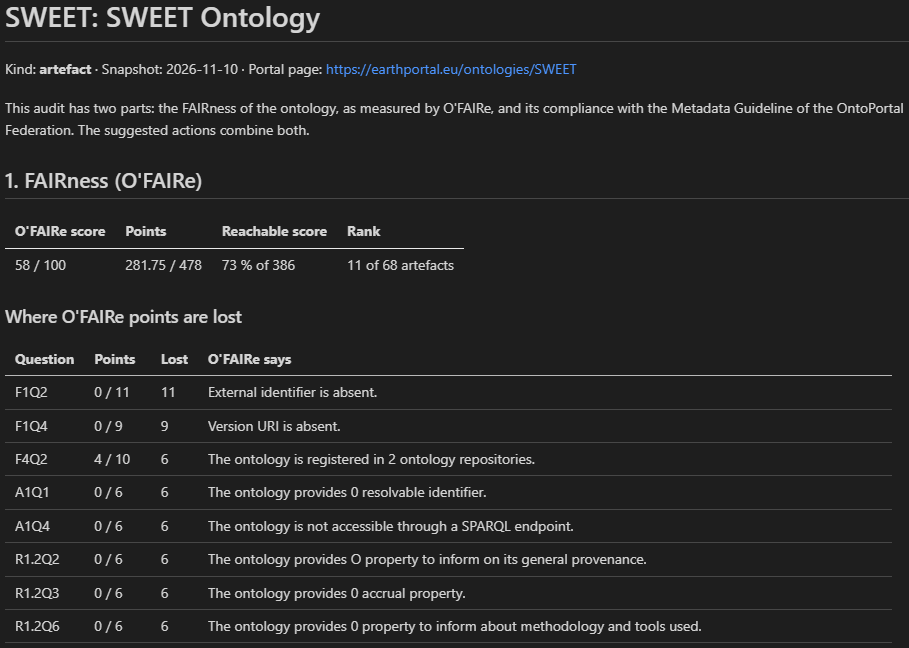
\includegraphics[width=0.95\textwidth]{Figures/slides_2026-11-13/SWEET_part1_crop.png}
    \end{column}
    \begin{column}{0.29\textwidth}
      \small
      Example: \textbf{SWEET}, the 11th artefact of the ranking.\\[6pt]
      Its scores, then every question where it loses points, largest loss first, with
      \textbf{O'FAIRe's own sentence}.
    \end{column}
  \end{columns}
  \vfill
  \evidence{\href{https://github.com/EarthPortal/SA_Management/blob/main/earthportal_sa_audit/audits/SWEET.md}{earthportal\_sa\_audit/audits/SWEET.md}, rendered by GitHub (snapshot of 10 November 2026).}
\end{frame}

% -----------------------------------------------------------------------------------------------------
\begin{frame}{One audit per artefact: 2. Your guidelines}
  \begin{columns}[c]
    \begin{column}{0.66\textwidth}
      \centering
      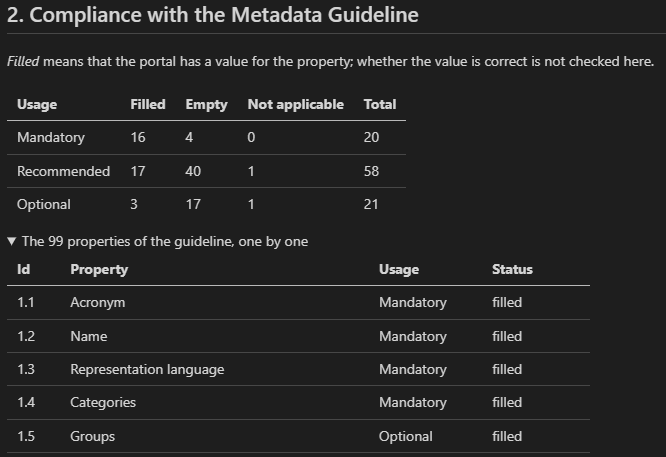
\includegraphics[width=\textwidth]{Figures/slides_2026-11-13/SWEET_part2_crop.png}
    \end{column}
    \begin{column}{0.31\textwidth}
      \small
      SWEET fills \textbf{16 of the 20} Mandatory properties, but only \textbf{17 of the 57}
      Recommended ones that apply.\\[6pt]
      The 99 properties are listed one by one in a folded block, each \emph{filled}, \emph{empty} or
      \emph{not applicable}.
    \end{column}
  \end{columns}
  \vfill
  \evidence{\emph{Not applicable}: \emph{This ontology is a view of} (only views) and \emph{Was invalidated by} (only retired artefacts).}
\end{frame}

% -----------------------------------------------------------------------------------------------------
\begin{frame}{One audit per artefact: 3. Actions, and after}
  \begin{columns}[T]
    \begin{column}{0.54\textwidth}
      \centering
      {\small\textbf{3. Suggested actions} (SWEET, first rows)}\\[2pt]
      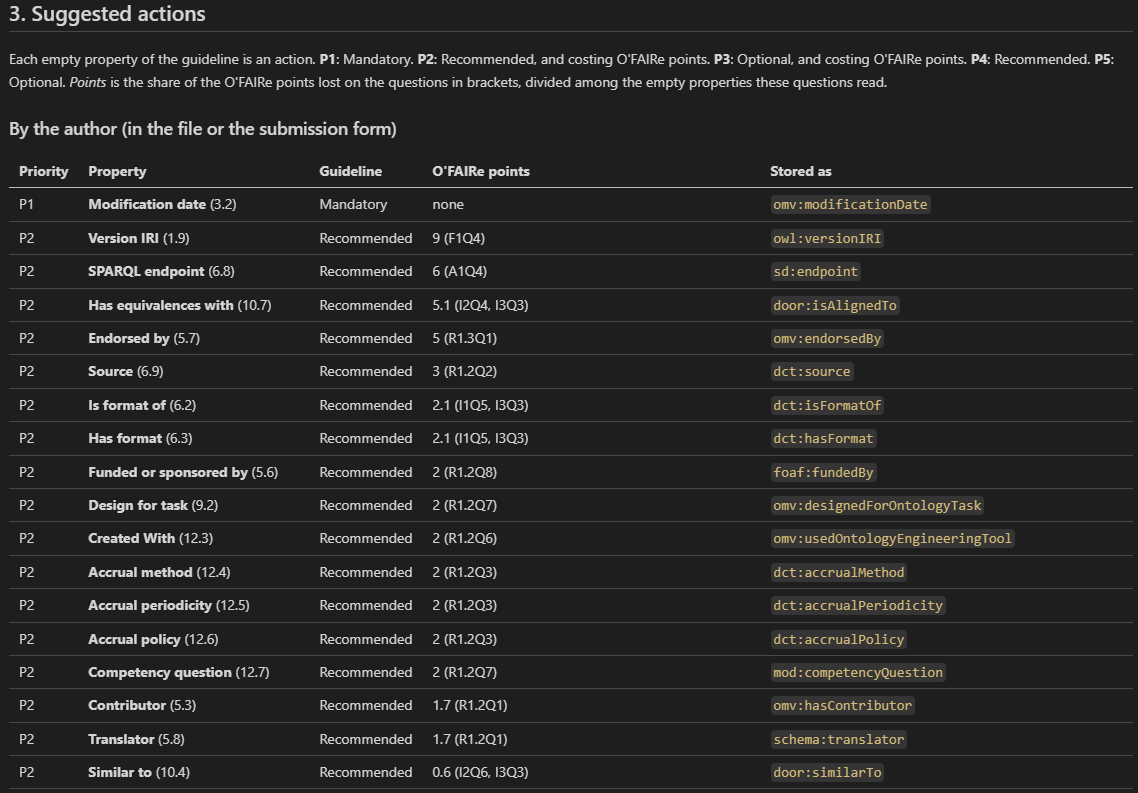
\includegraphics[width=\textwidth]{Figures/slides_2026-11-13/SWEET_part3_crop.png}
    \end{column}
    \begin{column}{0.43\textwidth}
      \small
      Each row says \textbf{why the guidelines ask} for the property and \textbf{what it is worth} in
      O'FAIRe.\\[6pt]
      \begin{block}{One JSON file per artefact}
        \scriptsize The same audit, as data: \code{audits/json/<ACRONYM>.json}. The page is written
        from it. It holds statuses, scores and actions, and no personal data.
      \end{block}
      \vspace{4pt}
      \begin{exampleblock}{A curation interface}
        \scriptsize Amine Kasmi (EarthPortal) is building a curation interface on these JSON files:
        work in progress (\href{https://github.com/EarthPortal/SA_Management/blob/main/docs/build/emmanuel_dataTerra_Report6-Curation-Interface.pdf}{Report 6}).
      \end{exampleblock}
    \end{column}
  \end{columns}
\end{frame}

% =====================================================================================================
\section{What we got on 10 November 2026}

% -----------------------------------------------------------------------------------------------------
\begin{frame}{How FAIR is the catalogue?}
  \begin{columns}[c]
    \begin{column}{0.56\textwidth}
      \centering
      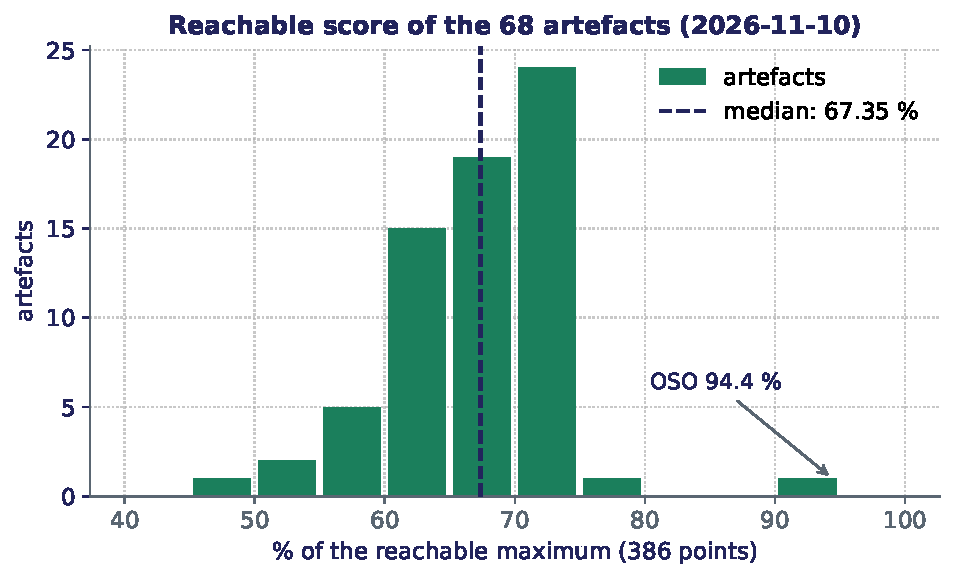
\includegraphics[width=\textwidth]{../earthportal_sa_audit/figures/fig_reachable_hist.pdf}
    \end{column}
    \begin{column}{0.42\textwidth}
      \small
      \textbf{68 artefacts}:
      \begin{itemize}
        \item reachable score: median \textbf{67.35\,\%}, from 49.5\,\% (STY) to 94.4\,\% (OSO)
        \item O'FAIRe's own score: median \textbf{54 / 100}
        \item one clear leader; most artefacts between 60 and 75\,\%
      \end{itemize}
      \vspace{4pt}
      \begin{block}{Between 16 October and 10 November}
        \scriptsize The status of the 99 properties is identical. Six scores
        moved only through O'FAIRe's live checks (for example SEWERNET $-3.9$, GEOLTSBOUND $+2.3$).
      \end{block}
    \end{column}
  \end{columns}
\end{frame}

% -----------------------------------------------------------------------------------------------------
\begin{frame}{How much of your guidelines is filled?}
  \begin{columns}[c]
    \begin{column}{0.56\textwidth}
      \centering
      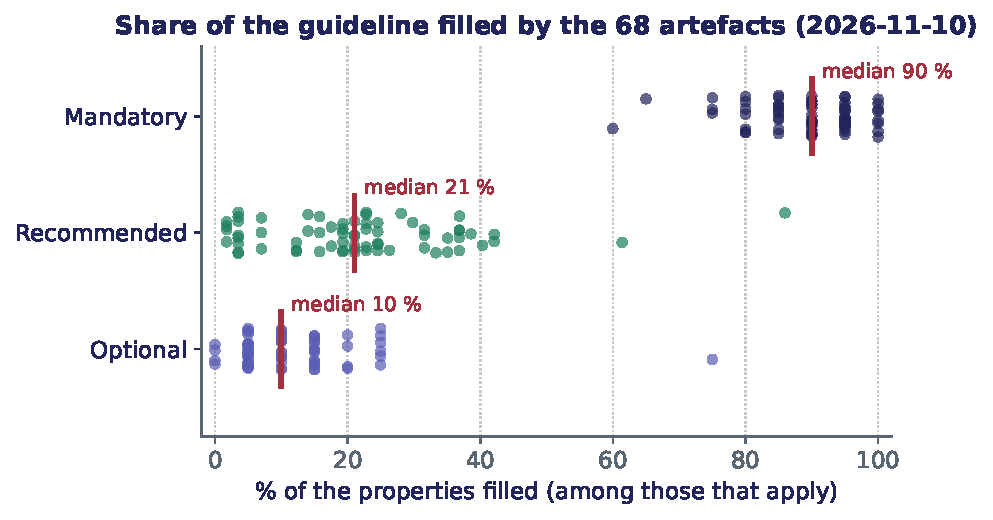
\includegraphics[width=\textwidth]{../earthportal_sa_audit/figures/fig_guideline_compliance.pdf}
    \end{column}
    \begin{column}{0.42\textwidth}
      \small
      Share of the properties filled, among those that apply, for each of the 68 artefacts:
      \begin{itemize}
        \item \textbf{Mandatory}: median \textbf{90\,\%}
        \item \textbf{Recommended}: median \textbf{21\,\%}
        \item \textbf{Optional}: median \textbf{10\,\%}
      \end{itemize}
      \vspace{4pt}
      \begin{alertblock}{Two stories}
        \scriptsize The median artefact reaches 67\,\% of what O'FAIRe can give, but fills only a fifth of
        what your guidelines recommend.
      \end{alertblock}
      \evidence{``Filled'' means present; the value is not checked.}
    \end{column}
  \end{columns}
\end{frame}

% -----------------------------------------------------------------------------------------------------
\begin{frame}{Where the catalogue loses most points}
  \begin{columns}[c]
    \begin{column}{0.60\textwidth}
      \centering
      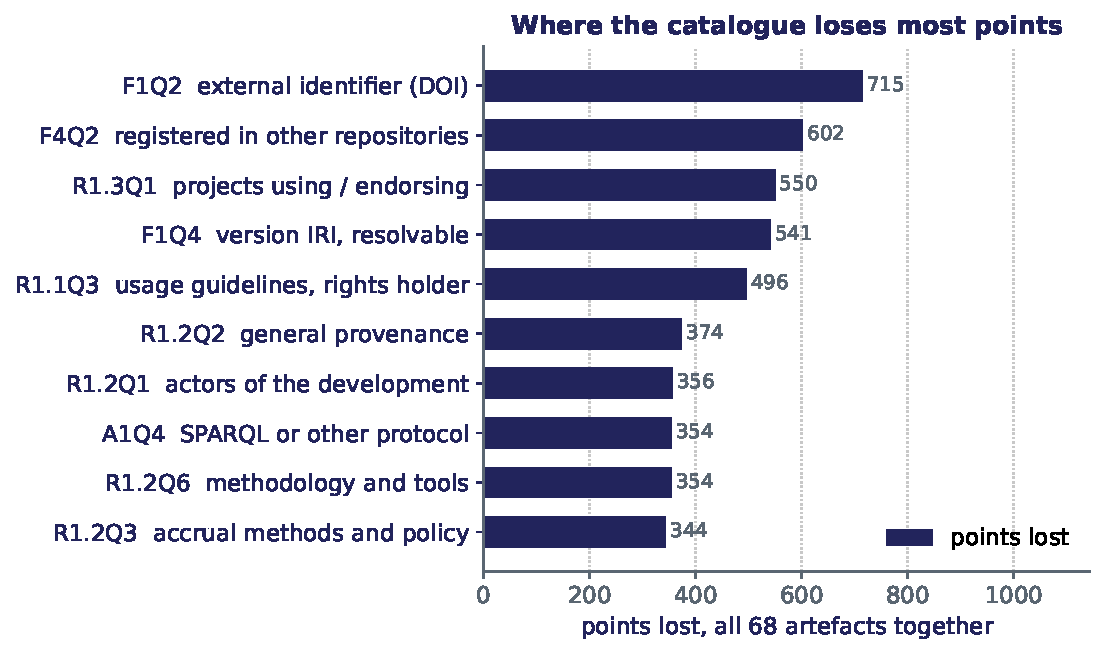
\includegraphics[width=\textwidth]{../earthportal_sa_audit/figures/fig_lost_points.pdf}
    \end{column}
    \begin{column}{0.38\textwidth}
      \small
      Points lost $= \sum_{o} (m_q - s_q(o))$ over the 68 artefacts.
      \begin{itemize}
        \item \textbf{F1Q2}: 65 artefacts have no external identifier; only a registered
              \textbf{DOI} gives the full 11 points
        \item \textbf{F4Q2}: EarthPortal is not in O'FAIRe's list of repositories
        \item \textbf{R1.3Q1}: 50 artefacts say nothing about projects using them or organisations
              endorsing them
      \end{itemize}
      \evidence{\emph{Other identifier} (a DOI) is the action with the largest share for 57 of the 68 artefacts.}
    \end{column}
  \end{columns}
\end{frame}

% -----------------------------------------------------------------------------------------------------
\begin{frame}{Who can act? Mostly the authors}
  \begin{columns}[c]
    \begin{column}{0.42\textwidth}
      \small
      \textbf{4\,378 actions} for the 68 artefacts:\\[4pt]
      \begin{tabular}{@{}l r r@{}}
        \toprule
        Who & P1 to P3 & All (P1 to P5)\\
        \midrule
        author & 2\,626 & 4\,163\\
        curator & 81 & 178\\
        portal & 37 & 37\\
        \bottomrule
      \end{tabular}\\[8pt]
      \begin{alertblock}{Preventing is better than curing}
        \scriptsize The submission form does not ask for the \textbf{licence}, the \textbf{creator} or the
        \textbf{modification date}, and \textbf{categories} are not required: four of the five
        Mandatory properties most often empty.
      \end{alertblock}
    \end{column}
    \begin{column}{0.56\textwidth}
      \centering
      {\small Mandatory properties most often empty}\\
      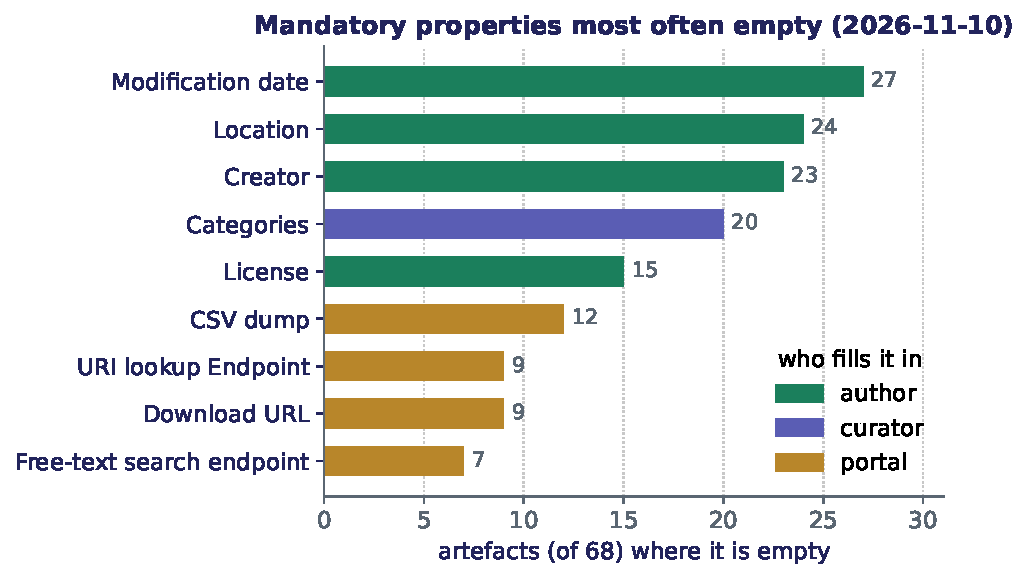
\includegraphics[width=\textwidth]{../earthportal_sa_audit/figures/fig_mandatory_empty.pdf}
    \end{column}
  \end{columns}
\end{frame}

% -----------------------------------------------------------------------------------------------------
\begin{frame}{The whole catalogue on one page}
  \begin{columns}[T]
    \begin{column}{0.58\textwidth}
      \centering
      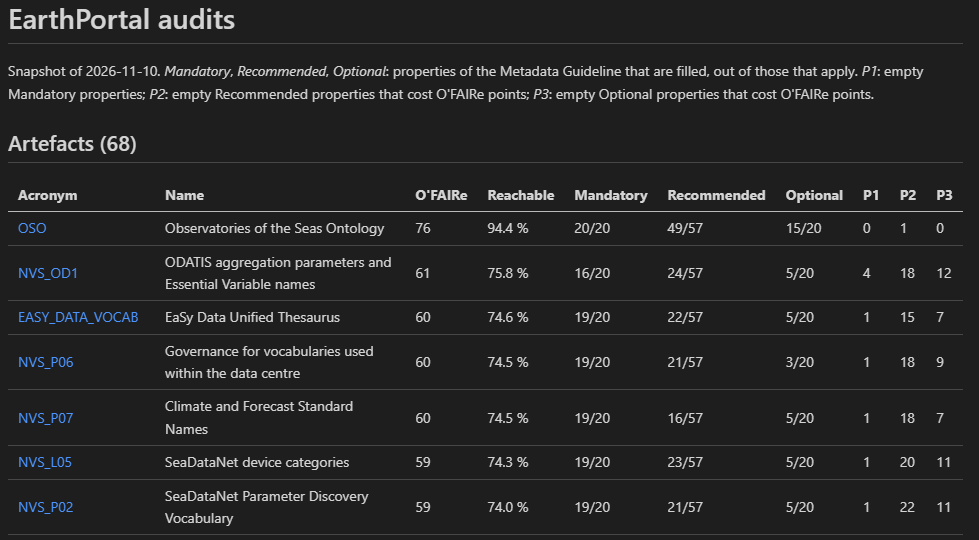
\includegraphics[width=\textwidth]{Figures/slides_2026-11-13/INDEX_top_crop.png}
    \end{column}
    \begin{column}{0.39\textwidth}
      \small
      \href{https://github.com/EarthPortal/SA_Management/blob/main/earthportal_sa_audit/audits/index.md}{\code{audits/index.md}}: every entry, best reachable score first, with its guideline properties
      filled and its P1 to P3 actions; each acronym opens its audit.\\[8pt]
      \begin{block}{Seen in the data}
        \scriptsize Two groups of artefacts give exactly the same answers to every question:
        DIVCHRONOSTRAT, DIVGEOCHRONO, GEOLTSBOUND, GEOLUNITTYPE; and TERRA\_VOCABS\_ESS,
        TERRA\_VOCABS\_ESV. Probably the same description template: worth a curator's look.
      \end{block}
    \end{column}
  \end{columns}
\end{frame}

% =====================================================================================================
\section{Reproducibility and reuse}

% -----------------------------------------------------------------------------------------------------
\begin{frame}{Open, reproducible and citable}
  \begin{columns}[T]
    \begin{column}{0.30\textwidth}
      \centering
      \qrcode[height=2.6cm]{https://github.com/EarthPortal/SA_Management}\\[4pt]
      \scriptsize\href{https://github.com/EarthPortal/SA_Management}{github.com/EarthPortal/SA\_Management}\\[2pt]
      MIT licence
    \end{column}
    \begin{column}{0.66\textwidth}
      \small
      \begin{itemize}
        \item \textbf{Dated snapshots.} Only notebook 01 uses the network; 02 to 05 always give the same
              results for the same date.
        \item \textbf{One setup.} Python 3.12+, one \code{requirements.txt}, one \code{.env} with your
              API key.
        \item \textbf{Explained for non-programmers.} Each notebook block comes with a plain-text explanation.
        \item \textbf{Citable.} Each GitHub release is archived on Zenodo with a DOI:\\
              software \href{https://doi.org/10.5281/zenodo.23417011}{10.5281/zenodo.23417011} (v1.0.0),
              slides \href{https://doi.org/10.5281/zenodo.23391527}{10.5281/zenodo.23391527}.
        \item \textbf{Documented.} \code{ARCHITECTURE.md} (structure), six short reports in \code{docs/}.
      \end{itemize}
    \end{column}
  \end{columns}
\end{frame}

% -----------------------------------------------------------------------------------------------------
\begin{frame}{Running the pipeline on another portal}
  \begin{columns}[T]
    \begin{column}{0.50\textwidth}
      \begin{exampleblock}{What stays the same}
        \small
        \begin{itemize}
          \item your guidelines (the cheatsheet) and the machine-readable profile
          \item the five notebooks and the audit format
          \item the reading of O'FAIRe
        \end{itemize}
      \end{exampleblock}
    \end{column}
    \begin{column}{0.46\textwidth}
      \begin{block}{What to change or check}
        \small
        \begin{enumerate}
          \item the portal's API, web address and O'FAIRe service in \code{.env}
          \item an API key of that portal
          \item the 6 manual links, if its schema differs
          \item the reachable maximum (386), which depends on the portal
        \end{enumerate}
      \end{block}
    \end{column}
  \end{columns}
  \vfill
  \evidence{Step by step in \href{https://github.com/EarthPortal/SA_Management/blob/main/ADAPTING.md}{\code{ADAPTING.md}}, at the root of the repository.}
\end{frame}

% -----------------------------------------------------------------------------------------------------
\begin{frame}{Limits, said plainly}
  \begin{columns}[T]
    \begin{column}{0.48\textwidth}
      \begin{block}{Presence, not correctness}
        \small A property counts as filled when it is not empty. Default values and wrong IRIs pass,
        in O'FAIRe and in our audits.
      \end{block}
      \begin{block}{Who fixes it}
        \small The split author / curator / portal is a proposal. No audit has been sent to an
        author yet.
      \end{block}
    \end{column}
    \begin{column}{0.48\textwidth}
      \begin{block}{O'FAIRe on the server}
        \small We read commit \code{24def6b}; we do not know which version runs on EarthPortal, nor
        how often its results are refreshed.
      \end{block}
      \begin{block}{The guidelines move}
        \small Our cheatsheet follows the review version of September 2026. A new version of the
        guidelines means a new cheatsheet, then a new run.
      \end{block}
    \end{column}
  \end{columns}
\end{frame}


% -----------------------------------------------------------------------------------------------------
\begin{frame}{Acknowledgements}
  \begin{columns}[T]
    \begin{column}{0.48\textwidth}
      \begin{block}{Christelle Pierkot}
        \small My supervisor, whose guidance and support made this pipeline, and its latest results,
        possible.
      \end{block}
      \begin{block}{Clément Jonquet}
        \small For O'FAIRe, and for spending a day with us at Data Terra to discuss it and the way
        we use it in this pipeline.
      \end{block}
    \end{column}
    \begin{column}{0.48\textwidth}
      \begin{block}{The Editorial Board}
        \small For welcoming me into your team, and for the Metadata Guidelines: the cornerstone
        (\emph{la pierre angulaire}) of this pipeline.
      \end{block}
      \begin{block}{The Data Terra team}
        \small Christelle, Nicolas, Hakim, Imene, Amirat, and Amine: a welcoming, supportive and dynamic team.
        It was a great honour and pleasure to work with you.
      \end{block}
    \end{column}
  \end{columns}
\end{frame}

% -----------------------------------------------------------------------------------------------------
% Thank you, with two QR codes: the software (concept DOI, always the latest release) and these
% slides (version DOI 10.5281/zenodo.24145898, reserved on Zenodo on 11 November 2026)
{\darkbackground
\begin{frame}[plain]
  \begin{tikzpicture}[remember picture,overlay]
    \node[text=white,font=\fontsize{24}{28}\selectfont\bfseries] at ($(current page.center)+(-3.7cm,1.85cm)$) {Thank you};
    \node[text=white,font=\normalsize,align=center] at ($(current page.center)+(-3.7cm,1.0cm)$)
      {Merci beaucoup $\cdot$ Vielen Dank\\[2pt] Grazie mille};
    \node[text=white,font=\small\itshape,align=center] at ($(current page.center)+(-3.7cm,-0.2cm)$)
      {``All models are wrong, but some are useful.''};
    \node[text=white!85,font=\scriptsize,align=center] at ($(current page.center)+(-3.7cm,-0.6cm)$) {George E.\ P.\ Box};
    \node[text=white,font=\small\itshape,align=center] at ($(current page.center)+(-3.7cm,-1.15cm)$) {``Big goals, small steps.''};
    \foreach \x/\file/\head/\doi in {
      1.75/QR_software_concept_DOI/Software/{10.5281/zenodo.23417011},
      5.45/QR_slides_Federation_version_DOI/{These slides}/{10.5281/zenodo.24145898}} {
      \node[fill=white,rounded corners=6pt,inner sep=5pt] at ($(current page.center)+(\x cm,0.75cm)$)
        {\includegraphics[width=2.2cm]{Figures/slides_2026-11-13/\file.png}};
      \node[text=white,font=\small\bfseries] at ($(current page.center)+(\x cm,-0.85cm)$) {\head};
      \node[text=white!85,font=\scriptsize] at ($(current page.center)+(\x cm,-1.25cm)$) {\doi};
    }
  \end{tikzpicture}
\end{frame}
}

% -----------------------------------------------------------------------------------------------------
\begin{frame}{Let's discuss}
  \begin{columns}[T]
    \begin{column}{0.50\textwidth}
      \begin{block}{About the guidelines}
        \small
        \begin{enumerate}
          \item The \textbf{five names} the portal does not recognise: change the guidelines, or
                declare new mappings in the portal?
          \item Add the \textbf{eight fields} O'FAIRe reads (version information, deprecated,
                object description properties), with their allowed values?
          \item Could the \textbf{machine-readable profile} be published and versioned with the
                guidelines?
        \end{enumerate}
      \end{block}
    \end{column}
    \begin{column}{0.46\textwidth}
      \begin{block}{About the portals and O'FAIRe}
        \small
        \begin{enumerate}
          \setcounter{enumi}{3}
          \item Should the submission form ask for the \textbf{licence}, the \textbf{creator}, the
                \textbf{modification date}, and require \textbf{categories}?
          \item Should \textbf{Location} stay Mandatory when a file is uploaded?
          \item Could EarthPortal, and the other portals of the Federation, be added to O'FAIRe's
                list of \textbf{repositories} (F4)?
        \end{enumerate}
      \end{block}
    \end{column}
  \end{columns}
\end{frame}

% =====================================================================================================
\appendix
{\shownumberfalse
\begin{frame}[noframenumbering]
  \centering
  {\color{epnavy}\fontsize{22}{26}\selectfont\bfseries Backup slides}
\end{frame}
}

% -----------------------------------------------------------------------------------------------------
\begin{frame}{The ten questions O'FAIRe does not implement}
  \scriptsize
  \begin{tabularx}{\textwidth}{@{}l r X@{}}
    \toprule
    Question & Max & Text\\
    \midrule
    F4Q3 & 8 & Are the ontology libraries or repositories properly indexed by Web search engines?\\
    I2Q3 & 3 & If yes, does it include the minimum information for those terms?\\
    I2Q5 & 7 & If yes, are those alignments well represented and to unambiguous entities? \dots\\
    I3Q1 & 20 & Does an ontology provide qualified cross-references to external resources/databases?\\
    I3Q2 & 6 & If yes, are those cross-references well represented and to unambiguous entities?\\
    R1Q3 & 7 & How much of the ontology objects are described with labels?\\
    R1Q4 & 6 & How much of the ontology objects are defined using a text description?\\
    R1Q5 & 6 & How much ontology objects are defined using a property restriction or an equivalent class?\\
    R1Q6 & 5 & How much of the ontology objects provide provenance information with annotation properties?\\
    R1.2Q5 & 2 & Are the ontology latest changes documented?\\
    \midrule
    \textbf{Total} & \textbf{70} & Every answer: ``This question cannot be evaluated in the repository at this time.''\\
    \bottomrule
  \end{tabularx}
\end{frame}

% -----------------------------------------------------------------------------------------------------
\begin{frame}{F4: the repositories O'FAIRe knows}
  \small
  F4Q1 and F4Q2 count the catalogues of \code{includedInDataCatalog} that appear in O'FAIRe's list
  (\code{catalogs.config.json}, commit \code{24def6b}): \textbf{23 repositories} and \textbf{13 libraries}.\\[6pt]
  \scriptsize
  \begin{tabularx}{\textwidth}{@{}l X@{}}
    \toprule
    Repositories & NCBO BioPortal, AgroPortal, SIFR BioPortal, EBI OLS, Ontobee, OntoHub, AberOWL, LOV, ONKI,
    MMI ORR, ESIP COR, LifeWatch EcoPortal, MatPortal, MedPortal, CISMeF HeTOP, FINTO, ANDC RVA, NVS, GFBIO TS,
    Loterre, Caliper, Crop Ontology Curation Tool, Planteome\\
    Libraries & OBO Foundry, Agrisemantics, FAIRsharing, ROMULUS, DAML Ontology Library, Colore, BARTOC,
    TaxoBank, LusTRE, LOV4IoT, VOCAB OEG, LiveSchema, Protégé Ontology Library\\
    \bottomrule
  \end{tabularx}\\[8pt]
  \small EarthPortal is not in the list, so an artefact hosted on EarthPortal does not get the point
  of ``its own'' portal (F4Q1), and the catalogue loses 602 points on F4Q2.
\end{frame}


% -----------------------------------------------------------------------------------------------------
\begin{frame}{Who fixes what? The split author / curator / portal}
  \centering
  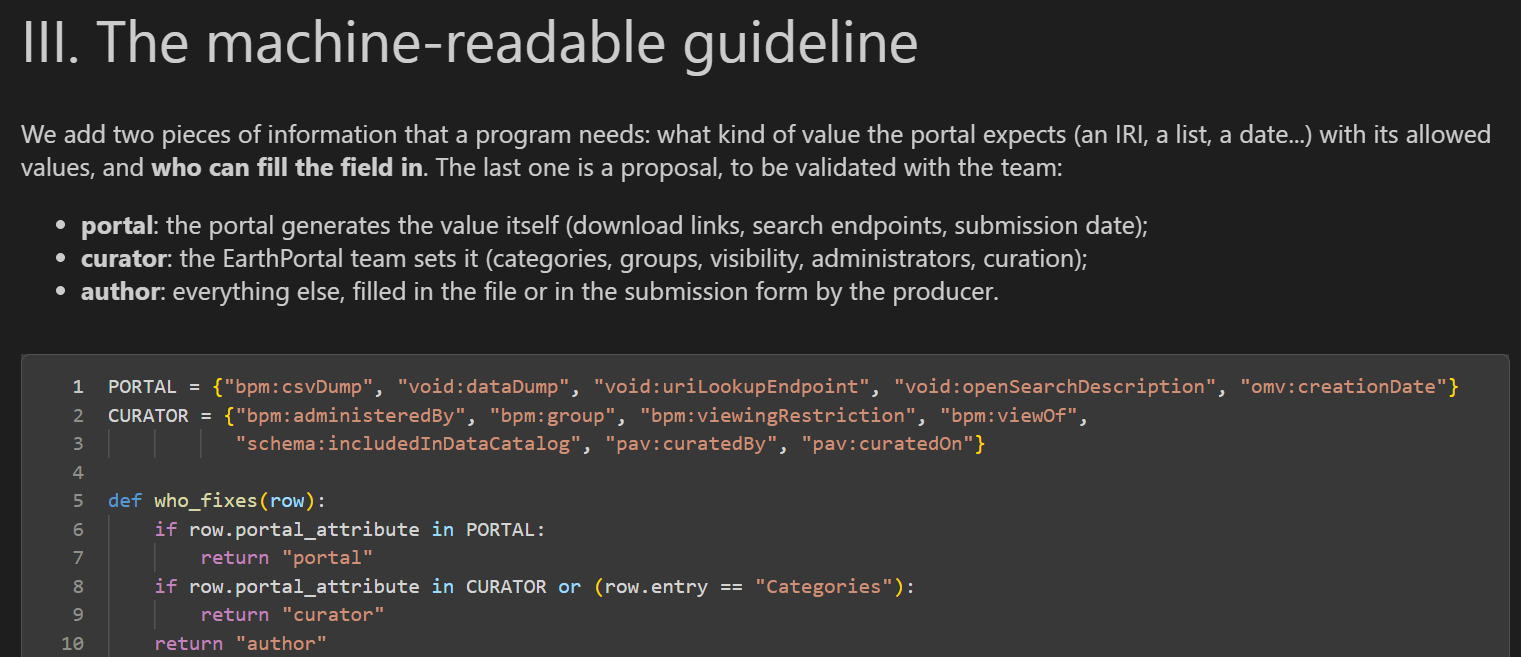
\includegraphics[width=0.95\textwidth]{Figures/slides_2026-11-13/whoFixes_metadataSchema.png}
  \vfill
  \evidence{Notebook: \href{https://github.com/EarthPortal/SA_Management/blob/main/earthportal_sa_audit/04_guideline_vs_ofaire.ipynb}{\code{04\_guideline\_vs\_ofaire.ipynb}.}}
\end{frame}

% -----------------------------------------------------------------------------------------------------
\begin{frame}{The snapshots so far}
  \small
  \begin{tabular}{@{}l c c c c c c@{}}
    \toprule
    Snapshot & Entries & Artefacts & Views & No content & Median reachable & OSO\\
    \midrule
    28 Sept 2026 & 91 & 70 & 16 & 5 & about 67\,\% & 93.9\,\%\\
    8 Oct 2026 & 92 & 68 & 19 & 5 & 67.85\,\% & 94.4\,\%\\
    16 Oct 2026 & 92 & 68 & 19 & 5 & 67.85\,\% & 94.4\,\%\\
    10 Nov 2026 & 92 & 68 & 19 & 5 & 67.35\,\% & 94.4\,\%\\
    \bottomrule
  \end{tabular}\\[10pt]
  \begin{itemize}
    \item early October: \code{OSO-DCAT}, \code{OSO-VOID} and \code{OSO-SHACL} became views of OSO
    \item 10 November: \textbf{6\,206 actions} for the 92 entries (P1 224, P2 2\,812, P3 999,
          P4 1\,517, P5 654)
  \end{itemize}
  \vfill
  \evidence{\code{earthportal\_sa\_audit/data/ofaire\_scores\_<date>.csv}: one file per snapshot.}
\end{frame}

\end{document}
